\chapter{Background}
\label{chapter:background}

%Positioning has been around since the need to locate warships arose. 
Technology has evolved and due to that, with the use of positioning methods, nowadays it is used to locate people and devices indoors. 

This chapter discusses about the knowledge needed prior to the implementation of an indoor positioning system. Section~\ref{section:Technologies} introduces the technologies used to calculate the position and achieve the positioning system referred in~\ref{section:objectives}, such as: \gls{gps}, \gls{wi-fi}, Bluetooth, \gls{qrcodes}, \gls{nfc} and \gls{rfid}.
In~\ref{section:methods}, several methods about positioning, for example Lateration and Fingerprinting, are introduced and then in~\ref{section:protocols} the latest beacons, its characteristics and limitations in indoor environments are going to be introduced. ~\ref{section:manufacturers} makes reference to the different types of beacons manufacturers on the market. In ~\ref{section:aplications} are commented the functionalities of the applications already existing in the market. The Section~\ref{section:summarybackground} does a summary about everything that was mentioned before.

%%%%%%%%%%%%%%%%%%%%%%%%%%%%%%%%%%%%%%%%%%%%%%%%%%%%%%%%%%%%%%%%%%%%%%%%

\section{Technologies}
\label{section:Technologies}
Mobile devices must be able to calculate their position, using a specific technology, in order to be used in a positioning system. Several types of technologies can obtain the position of a device in an indoor environment.
The most well-known technologies for positioning are introduced below with the corresponding advantages and limitations for its use in indoor systems.

\subsection{GPS}
\label{subsection:gps}

\gls{gps}\footnote{http://www.gps.gov} is a satellite system that is used to provide geolocation and time information to a \gls{gps} receiver anywhere on Earth.
In order to work correctly, in other words, without signal weakens or distortions making the result inaccurate, \gls{gps} receivers need to have a line of sight to four or more \gls{gps} satellites.

\gls{gps} uses trilateration as the technique to get the position of the receiver. With a view to calculate the position, the receiver needs the location of the satellites and the distance from the receiver to each one of those satellites. \gls{gps} receiver measures the distance to a \gls{gps} satellite using the travel time of radio signals.

The current \gls{gps} consists of three segments: the space segment, the control segment and the user segment.
The user segment is the part of the \gls{gps} system the user is most aware of. It is often simply equated with a \gls{gps} receiver, which is, only a part of the user segment. Its configuration actually depends on the application it is used for~\citep{KupperAxel}.
\gls{gps} is one of the most successful and popular positioning systems in outdoor environments. 

Despite being popular, it is not appropriate to indoor environments because microwaves will be attenuated and scattered by roofs, walls and other objects making it unsuitable for indoor positioning estimation due to its low accuracy. 

%An example of the malfunction in the use of \gls{gps} in indoor location applications, is one of the most downloaded applications in App Store history: Pokémon Go\footnote{http://www.pokemongo.com}. While playing the game indoor, a warning would appear saying that the user would be driving without even moving - this event is called \gls{gps} drift.

Another limitation of \gls{gps}, is the fact that it cannot detect altitude, being impossible to distinguish different floors.

Therefore, some studies were made in order to improve indoor positioning with \gls{gps}, using \gls{gps} repeaters. However, the cost of installing these repeaters was high and the accuracy did not improve as much as expected~\citep{GPStransmitters}.

%%%%%%%%%%%%%%%%%%%%%%%%%%%%%%%%%%%%%%%%%%%%%%%%%%%%%%%%%%%%%%%%%%%%%%%%
\subsection{Wi-Fi}
\label{subsection:wifi}
\gls{wi-fi}\footnote{http://www.wi-fi.org} is a technology that enables devices to connect to a \gls{wlan} using radio waves.

It is based on the \gls{ieee} 802.11 standard.
\gls{wi-fi} compatible devices connect to the Internet via a wireless access point which does the access to a \gls{wlan} network. 

This technology is widely used all over the world and is one of the most common local area networking techniques today.

However, its use to indoor positioning brings several problems to the users, such as:

\begin{itemize}
\item Limitation of the update rate due to the increased duration of passive \gls{wi-fi} scans- where the device waits for a \gls{ssid};

\item Reducing \gls{wi-fi} throughput, increasing network traffic as well as reducing privacy due to the use of frequent active Wi-Fi scans, where the device to be positioned broadcasts a query;

\item \gls{wi-fi} does not require the signal strength value to be reported in any specific unit, which several positioning methods depend on. Because of this, some mobile platforms have not allowed the access to the \gls{wi-fi} scan data. For instance, Apple’s \gls{ios} only allows \gls{rss} readings from the connected access point~\citep{fingerprintingble}, making it impossible to use more advanced positioning methods to calculate the position.
\end{itemize}

\subsection{Bluetooth}
\label{subsection:bluetooth}
Bluetooth\footnote{https://www.bluetooth.com} is a wireless standard technology that connects devices, fixed or mobile, together over short distances and is becoming more and more popular in modern technologies. It can be found in all sorts of devices and areas of consumer goods from mobile phones, headsets, tablets, etc. 

Bluetooth technology was created as an open standard to allow connectivity between different products leading to a cooperation between industries.

The Bluetooth \gls{sig} manages the development of Bluetooth standards and the licensing of the Bluetooth Technologies. Since Bluetooth technology is built upon a core specification and layered with different services, the \gls{sig} has worked to ensure its interoperability. 

In order to achieve better values of power consumption, Bluetooth suffered an update to Bluetooth 4.0 where it included \gls{ble}, gaining a lot of attention in the Internet of Things concept.

\gls{ble} is the power consumption and application friendly version of Bluetooth built for the \gls{iot}. \gls{ble} has a standard wireless protocol that allows for multi-vendor interoperability and has several power consuption modes, such as: ultra-low peak, average and idle mode that gives the ability to run for several months on a standard coin-cell battery.

\gls{ble} communication works in two different modes: advertising and connection.
Advertising is a one-way discovery mechanism. Devices which want to be discovered transmit packets of data repeatedly in intervals of time. The shorter the interval, the shorter the battery life is going to be and the faster the device can be discovered.
\gls{ble} devices can operate in advertisement mode only, in which all the information is contained in the advertisement.

\subsection{QR Codes}
\label{subsection:qrcodes}
\gls{qrcodes} are a two-dimension bade code which can be read by an application downloaded on a mobile device, that uses the camera to collect and then decode the data from the image. 

\gls{qrcodes} can be used to link the user directly to a \gls{url}, send a text message, call a phone number, decode a secret message or download contact information. QR codes can be freely generated in the Internet.

To read a small size QR code, for example a QR code in a magazine, the device should be at a maximum distance of 10 centimetres. \gls{qrcodes} can also be read from further away but their size should increase, for example, \gls{qrcodes} on sign posts or buildings must be scanned in a distance between 3 and 8 meters.

However, one limitation of this technology is the fact that it requires user interaction, that means the user needs to be aware of this codes to collect them.

\subsection{NFC}
\label{subsection:nfc}
\gls{nfc}\footnote{http://nearfieldcommunication.org} is a contactless form of communication between devices because it allows the user to send information over a \gls{nfc} compatible device, without needing to place the devices together or through several steps to make a connection. 

\gls{nfc} transmissions can occur in two modes: active and passive.
In the active mode, both devices generate the radio signal.
In Passive, only one device generates the radio signal of the connection and the second is powered by this. This mode can be used on items that do not need to receive direct power.

As in \gls{qrcodes}, to use \gls{nfc} the user needs to be aware of this devices because \gls{nfc} has a very short range, up to 4 or 5 centimetres. The need for a reader is another limitation of this type of technology.


\subsection{RFID}
\label{subsection:rfid}
\gls{rfid} is a technology that uses radio frequency signals to capture data. The method of identification in \gls{rfid} consists in storing a serial number that identifies an object or a person, on a microchip.

An \gls{rfid} system has several basic components, including \gls{rfid} readers, \gls{rfid} tags and the communication between them.

The read range of \gls{rfid} tags vary, some tags can be read from 30 meters and others only from 10 centimetres. 

\gls{rfid} tags can be categorized, as \gls{nfc}, in two categories: active or passive, depending if they operate with or without battery.

\subsection{Comparison}
\label{subsection:comparisontechnologies}

After introducing these technologies, it is possible to make a comparison between them, with the objective of exposing their differences to help in further technology selection in terms of cost, accuracy, precision, complexity, scalability and robustness. \gls{nfc} and \gls{qrcodes} present the same characteristics as \gls{rfid} which was the chosen technology from the three to be compared with the others.
This comparison can be seen in Table~\ref{tab:technodif}~\citep{SurveyofWireless}.

%%%%%%%%%%%%%%%%%%%%%%%%%%%%%
\begin{table}[!htb]
  \renewcommand{\arraystretch}{2} % more space between rows
  \centering
  \resizebox*{\textwidth}{!}{
  \begin{tabular}{lccccc p{1.5cm}}
    \toprule
   \textbf{Technologies} &Accuracy&Precision&Scale&Complexity&Robustness&Cost\\
    \midrule
    \textbf{GPS}   		&5m-50m&50\% within 25m&Good&High&Poor&Medium \\
    \textbf{Wi-Fi}		&3~5m&50\% within 2.5m and 90\% within around 5.9m&Good&Moderate&Good&Low\\
    \textbf{Bluetooth}	&2m&95\% within 1m&Nodes placed every 2-15m&positioning delay 15-30s&Poor&Medium\\
    \textbf{RFID}		&$<$2m&50\% within 1m&Nodes placed densely&Medium&Poor&Low\\
    \bottomrule
  \end{tabular}
  }
  \caption[Technologies' Differences]{Technologies' Differences.}
  \label{tab:technodif}
\end{table}

%%%%%%%%%%%%%%%%%%%%%%%%%%%%%%%%%%%5
\section{Positioning Methods}
\label{section:methods}
Several methods can be used to estimate the position of devices. The estimation can use one or more methods. In this section the necessary measures and methods for the realization of the estimation are approached.
A lot of measurements can be used to calculate the position of a device, such as \gls{aoa}, \gls{tof} and \gls{rss}, Received Signal Strength. However, mobile devices do not support the hardware necessary to obtain some types of measurements, for instance, the \gls{aoa} of the received signal. In indoor systems, due to its short distance, it is not appropriate to use the \gls{tof} of a signal because the time difference between sending and receiving is very small. 
\gls{rss} is an effective measure to the calculation of a position in an indoor system and it can be collected in mobile devices.


\subsection{Received Signal Strength}
\label{subsection:receivedsignal}
\gls{rss} can be used to calculate the distance, calculating the path loss when the signal travels from the sender to the receiver. The simplest model is the Friis free space model equation, which allows the consideration of environmental parameters only in the form of the path-loss gradient. \gls{rssi} can be calculated with the equation in~\ref{eq:rssi}.
\begin{equation}
\label{eq:rssi}
RSSI = -(10\cdot n)\log_{10}(d) +A
\end{equation}

\gls{rssi} in $dBm$, $n$ is the signal propagation constant, $d$ is the distance between the sender and the receiver and $A$ is the reference received signal strength in $dbm$ for the distance of one meter.
Equation~\ref{eq:distance} used to calculate the distance can be derived from~\ref{eq:rssi}.

\begin{equation}
\label{eq:distance}
d =10^{\frac{RSSI-A}{-10\cdot n}}
\end{equation}

In indoor environments, due to the short distances, can be really hard to measure the travelling time from the sender to the receiver, so the most used methods use \gls{rssi} values.

The methods of positioning to locate devices can be divided into two groups: active and passive~\citep{surveylocation}. 
Active positioning techniques determine the position of a device based on signals received.
Passive positioning techniques determine the position based on the information that the main sensor receives indirectly  from the environment. 


\subsection{Proximity Sensing}
\label{subsection:proximity}
Proximity Sensing is an active positioning technique and is the easiest and most widespread method to obtain the position of a target. It relies on the limited range of radio, infrared or ultrasound signals coverage.

In indoor systems, proximity sensing has been implemented in various research projects, since its accuracy works better for this kind of systems. The position of the terminal is determined from the position of the access point from which the terminal receives a greater \gls{rss} signal.

\subsection{Lateration}
\label{subsection:lateration}
Lateration is an active process of estimating the position of the target by measuring the distances to a set of points with a known location. The position is estimated using geometric figures such as circles, triangles or spheres. In order for the position to be estimated, at least three different base stations are needed. When the number of base stations used is three, lateration is also known as trilateration showed in Figure~\ref{fig:trilaterationimag}.

Suppose there are three distinct reference nodes  $p_{i}=
\left ( x_{i},y_{i} \right ),i =1,2,3$ in a two dimensional space and the coordinate 
$\left ( x_{0},y_{0} \right ) $ of an unknown node $p$ is going to be calculated, using $r_{i},i =1,2,3$.

\begin{figure}[!htb]
  \centering
  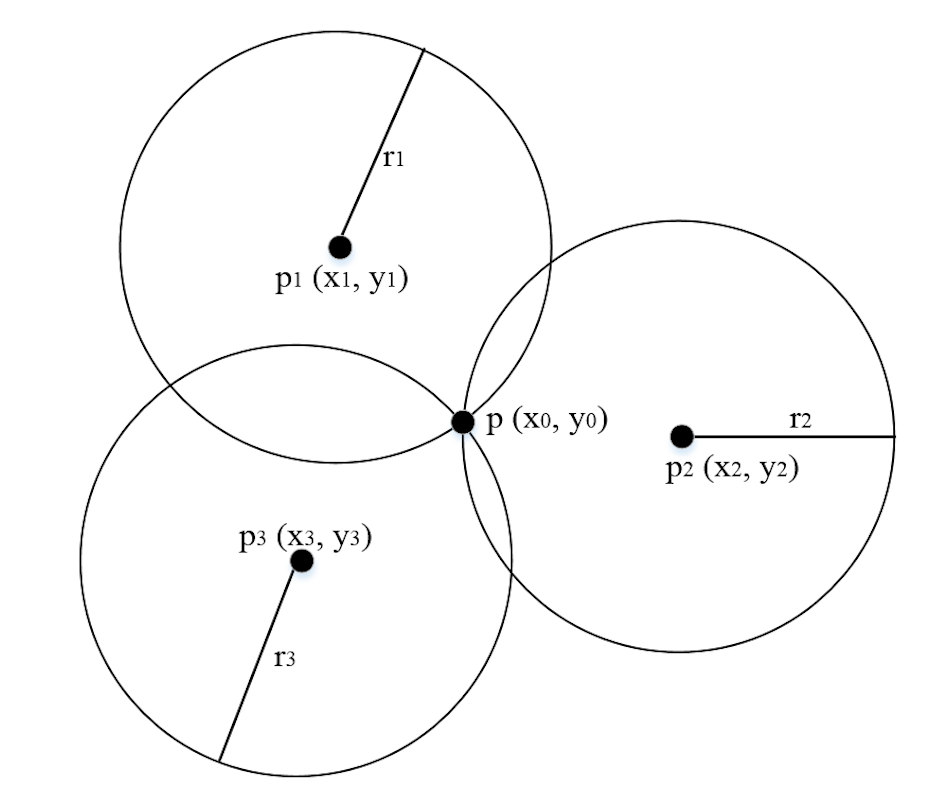
\includegraphics[width=0.5\textwidth]{Figures/trilat.png}
  \caption[Trilateration]{Trilateration}
  \label{fig:trilaterationimag}
\end{figure}

The following system of equations based on trilateration method is obtained:
\begin{equation}
\begin{cases} 
\left (x_{0}-x_{1}\right )^{2}+
\left (  y_{0}-y_{1}\right )^{2}={r_{1}}^{2}\\
\left (x_{0}-x_{2}\right )^{2}+\left (  y_{0}-y_{2}\right )^{2}={r_{2}}^{2}\\
\left (x_{0}-x_{3}\right )^{2}+\left (  y_{0}-y_{3}\right )^{2}={r_{3}}^{2}
\end{cases}
\end{equation}
From the previous system of equations the position of the unknown node $p$ is derived:
\begin{equation}
\begin{cases} 
x_{0} =\frac{1}{\Delta}\left ( 2T_{1}\left ( y_{1}-y_{3} \right )-2T_{2}\left ( y_{1}-y_{2} \right ) \right )
\\y_{0} =\frac{1}{\Delta}\left ( 2T_{2}\left ( x_{1}-x_{2} \right )-2T_{1}\left ( x_{1}-x_{3} \right ) \right )
\end{cases}
\end{equation}
where $ T_{1} = {r_{2}}^{2}-{r_{1}}^{2}-{x_{2}}^{2}+{x_{1}}^{2}-{y_{2}}^{2}+{y_{1}}^{2}
, T_{2} = {r_{3}}^{2}-{r_{1}}^{2}-{x_{3}}^{2}+{x_{1}}^{2}-{y_{3}}^{2}+{y_{1}}^{2}
$ and 
$\Delta  = 4\left ( \left ( x_{1}-x_{2} \right ) \left ( y_{1}-y_{3} \right )-\left ( x_{1}-x_{3} \right )\left ( y_{1}-y_{2} \right )\right )$.

The position of the target can only be estimated if the three nodes are not in a straight line. Moreover, the nodes should not be close to each other, otherwise $\Delta$ will become too small to estimate the unknown node~\citep{novelref}.

\subsection{Angulation}
\label{subsection:angulation}
Angulation is an active process of estimating the position of the target by using the angles between known base stations and the mobile device. To estimate the position, at least two base stations are needed. However, it is required that either base stations or terminals are equipped with antenna arrays. Suppose two distinct reference nodes exist $p_{i}=\left ( x_{i},y_{i} \right ),i =1,2$ using the angles $\alpha_{i}, i=1,2$ it is possible to estimate the position of the an unknown node $p$ as depicted in Figure~\ref{fig:angulation}~\citep{KupperAxel}.
\begin{figure}[!htb]
  \centering
  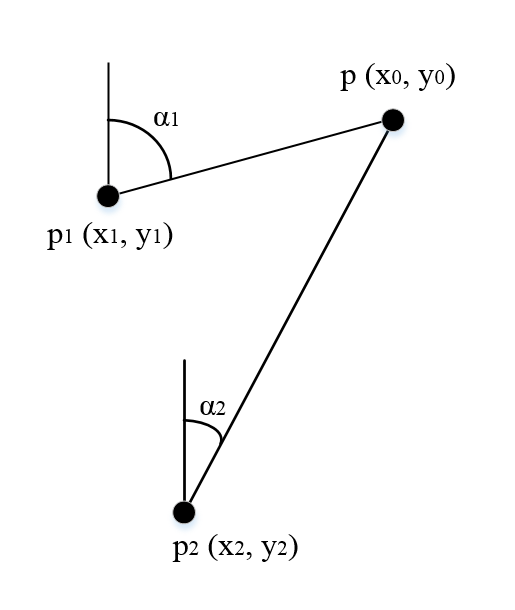
\includegraphics[width=0.3\textwidth]{Figures/ang.png}
  \caption[Angulation]{Angulation.}
  \label{fig:angulation}
\end{figure}

\subsection{Fingerprinting}
\label{subsection:fingerprinting}
Fingerprinting is a passive localization method and can be divided in two phases.

In the first phase, it is necessary to collect the \gls{rssi}, Radio Signal Strength Indicator, data along the locations where the user is expected to be, in order to construct a map of \gls{rssi} values, making this method environment related. These values are then stored in the fingerprinting database so that they can be used later. 
 
In the second phase, the device collects the \gls{rssi} values and compares them with the values in the fingerprinting database, to identify the values which relate the most to those obtained. Several methods of comparison can be used, such as: probabilistic methods, k-Nearest Neighbours, neutral networks, support vector machine and smallest M-vertex polygon~\citep{ImprIndoorLocal}.

	
\section{Beacons Protocols}
\label{section:protocols}
Beacons are small devices which only use the advertisement mode in \gls{ble}. They transmit packets of data in regular intervals of time, which can be then received by other devices like smartphones. The emitted message contains information that the receiving device can use to identify the beacon and to compute its relative distance to the beacon. The receiving device may use this information as a contextual trigger to execute procedures and implement behaviours that are relevant to being in proximity to the transmitting beacon.

There are several beacon protocols that define a message format for beacon advertisements, such as: 
\begin{itemize}
\item iBeacon,
\item AltBeacon,
\item Eddystone,
\item URIbeacon.
\end{itemize}

\subsection{iBeacon}
\label{subsection:ibeacon}
iBeacon\footnote{https://developer.apple.com/ibeacon/} is a protocol developed by Apple and was the first beacon protocol in the market. iBeacon works with Apple's \gls{ios} and Google's Android. It is widely supported, simple and easy to implement and has a reliable performance on \gls{ios}.
iBeacon broadcast segments of data, displayed in Figure~\ref{fig:ibeaconadv}, such as:
\begin{itemize}
\item iBeacon Prefix, containing the hexadecimal data: 0x0201061AFF004C0215.
\item \gls{uuid}, that identifies the beacon.
\item Major number, that identifies a subset of beacons within a large group.
\item Minor number, that identifies a specific beacon.
\item \gls{tx} power level in 2's complement, indicating the signal strength one meter from the device. This number must be calibrated for each device by the user or manufacturer. \gls{tx} power field is used with the measured signal strength to determine how far away the beacon is from the smart phone~\citep{smartanaibeacon}.
\end{itemize}

\begin{figure}[!htb]
  \centering
  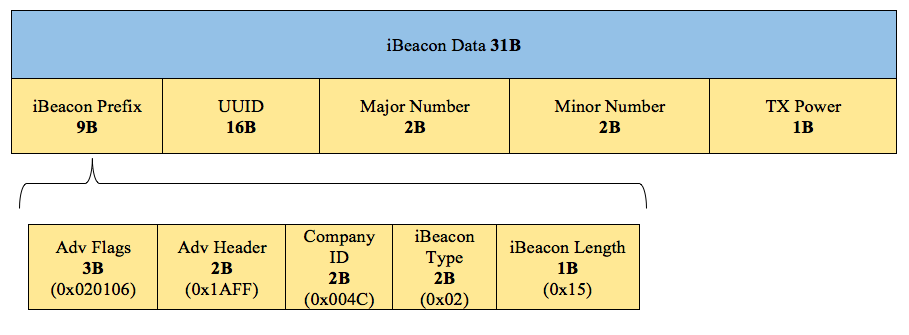
\includegraphics[width=1\textwidth]{Figures/ibeacon_v2.png}
  \caption[iBeacon Advertisement Format]{iBeacon Advertisement Format.}
  \label{fig:ibeaconadv}
\end{figure}

\subsection{AltBeacon}
\label{subsection:altbeacon}
AltBeacon\footnote{http://altbeacon.org} is a protocol specification provided by Radius Networks that defines a message format for proximity beacon advertisements. 
The AltBeacon advertisement makes use of the Manufacturer Specific Advertising Data structure as defined in Bluetooth 4.0, Volume 6, Part B, Section 2.3 Advertising Channel \gls{pdu}~\citep{roleofble_altbeacon}.
The AltBeacon advertisement, shown in Figure~\ref{fig:altbeaconadv}, is made up of:
\begin{itemize}
\item 1-byte length field;
\item 1-byte type field;
\item 2-byte company identifier, as prescribed by the Manufacturer Specific Advertising Data structure format;
\item 24 bytes containing the beacon advertisement data.
\end{itemize}

\begin{figure}[!htb]
  \centering
  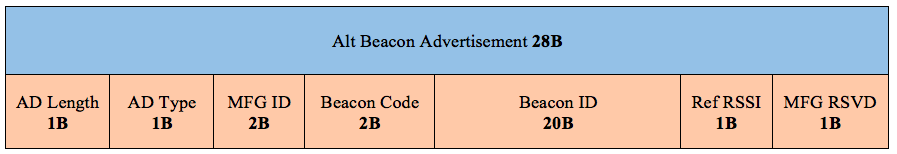
\includegraphics[width=1\textwidth]{Figures/altbeacon_v2.png}
  \caption[AltBeacon Advertisement Format]{AltBeacon Advertisement Format.}
  \label{fig:altbeaconadv}
\end{figure}

\subsection{Eddystone}
\label{subsection:eddystone}
Eddystone\footnote{https://github.com/google/eddystone} is an open beacon protocol developed by Google and designed with transparency. It can be detected by both Android and \gls{ios} devices. Eddystone protocol builds on lessons learned from working with industry partners in existing deployments, as well as the wider beacon community. Eddystone can have different types of payloads in the frame format, shown in Figure~\ref{fig:eddystoneadv}, such as:
\begin{itemize}
\item Eddystone-UID: A unique, opaque ID with a 10-byte Namespace component and a 6-byte Instance component. 
\item Eddystone-URL: A compressed \gls{url} that, once parsed and decompressed, is directly usable by the client. 
\item Eddystone-TLM: Beacon status data that is useful for beacon fleet maintenance, and powers Google Proximity Beacon \gls{api}'s diagnostics endpoint. -TLM should be interleaved with an identifying frame such as Eddystone-UID or Eddystone-EID (for which the encrypted eTLM version preserves security). 
\item Eddystone-EID: A time-varying beacon frame that can be resolved to a stable identifier by a linked resolver, such as Proximity Beacon \gls{api}~\citep{campus_survey}. 
\end{itemize}

\begin{figure}[!htb]
  \centering
  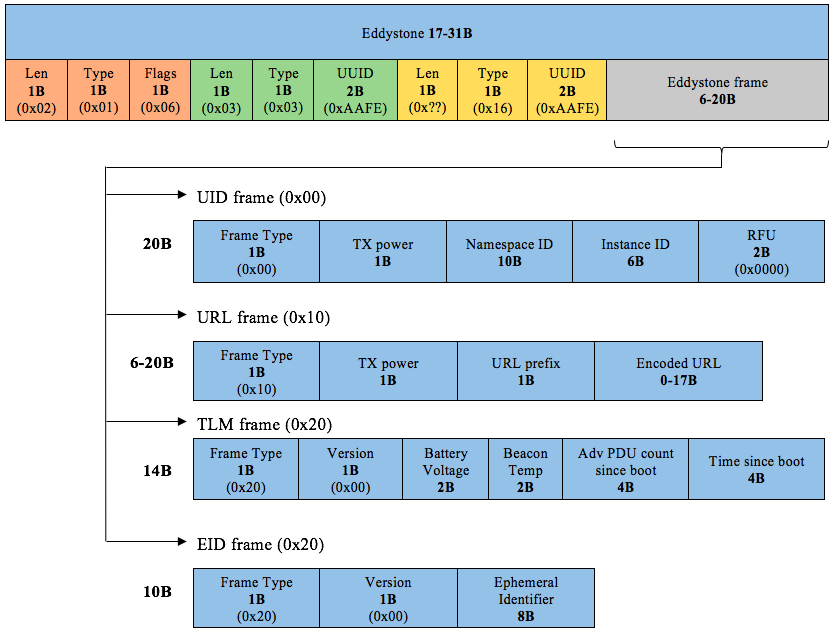
\includegraphics[width=1\textwidth]{Figures/eddystone_v3.png}
  \caption[Eddystone Advertisement Format]{Eddystone Advertisement Format.}
  \label{fig:eddystoneadv}
\end{figure}

\subsection{URIbeacon}
\label{subsection:uribeacon}
URIBeacon\footnote{https://github.com/google/uribeacon} is an open beacon protocol developed by Google and is part of Google’s project Physical Web initiative. URI beacon uses the payload to give short links to the internet via \gls{ble} advertising packets. The beacons using this protocol are meant to be updated with new information over time. Since they provide a link to the internet, they do not need a database to give meaning to the information they send. The URIBeacon advertisement format is displayed in the Figure~\ref{fig:uribeaconadv}.

\begin{itemize}
\item 19 bytes are used to encode the \gls{uri}.
\item The prefix and the suffix are encoded in two bytes. However, limiting the number of bytes only allows certain domains to be encoded. URIbeacons are supposed to be used with \gls{url} shortening services like goo.gl, bit.ly, tin.ly which will shorten any long \gls{url} to eight to ten bytes.
\end{itemize}
 

\begin{figure}[!htb]
  \centering
  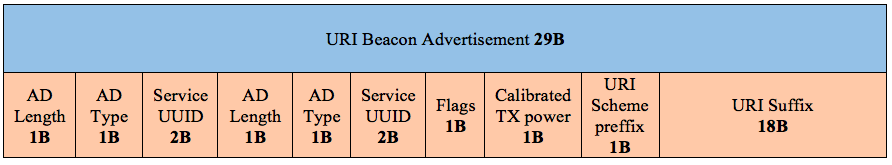
\includegraphics[width=1\textwidth]{Figures/uribeacon_v2.png}
  \caption[URIbeacon Advertisement Format]{URIbeacon Advertisement Format.}
  \label{fig:uribeaconadv}
\end{figure}

\subsection{Comparison}
\label{subsection:comparison}

After introducing these protocols, it is important to identify the biggest differences between them, which allows to choose between the protocol that makes the most sense to use in a project. These differences are summarized in the Table~\ref{tab:protocolsdif}.

\begin{table}[!htb]
  \renewcommand{\arraystretch}{2} % more space between rows
  \centering
  \resizebox*{\textwidth}{!}{
  \begin{tabular}{lcccc p{1.5cm}}
    \toprule
   \textbf{ Protocols      } &iBeacon&Eddystone&AltBeacon&URIBeacon\\
    \midrule
    \textbf{Developed by}    &Apple&Google&Radius Networks&Google\\
    \textbf{Open }			&No&Yes&Yes&Yes\\
    \textbf{Compatibility}	&\begin{tabular}[t]{@{}c@{}}Android and iOS,\\ but native only for iOS.\end{tabular}&Android and iOS.&Android and iOS.& Android and iOS.\\
    \textbf{\begin{tabular}[t]{@{}c@{}}Types of data \\broadcasted\end{tabular}}  & Unique ID number.&\begin{tabular}[t]{@{}c@{}}Unique ID number, or a URL \\address or sensor telemetry.\end{tabular}& Unique ID number.&Uniform Resource Identifier (URI).\\
    \textbf{API	}	&None&\begin{tabular}[t]{@{}c@{}}Nearby API, Proximity Beacon\\API and  Places API\end{tabular}&Android Library API&Same as Eddystone\\
    \bottomrule
  \end{tabular}
  }
  \caption[Beacons Protocols.]{Beacons Protocols.}
  \label{tab:protocolsdif}
\end{table}

The protocols can be divided in two groups where an ID number or an \gls{url} is broadcasted. iBeacon and AltBeacon are integrated in the group where an ID number is broadcasted and URIBeacon is integrated in the group where an \gls{url} is broadcasted. Eddystone can integrate both groups.

These two groups work in different ways:
\paragraph{ID number broadcasted}
\label{paragraph:sidnumber}
A scanning application reads the ID number and compares it with a database to get information about the beacon.
The beacon itself carries no descriptive information - it requires external database to be used. 

\paragraph{URL broadcasted} 
\label{paragraph:urlbroadcasted}
A scanning application reads the \gls{url} and opens it in a browser, it does not need a database to get the information.
The beacon information that is broadcasted in this case needs to be updated regularly.

\section{Manufacturers}
\label{section:manufacturers}
There is a wide variety of beacon manufacturers on the market. To choose the most appropriate beacon some criteria must be followed:
\begin{itemize}
\item Battery life and its rechargeability; 

\item Transmission rate and power.

\end{itemize}
The most common beacon manufacturers in the market are: Estimote, Gimbal, Bluvision and Kontakt.io~\citep{Statler}. Despite the existence of these well-known manufactures, other manufacturers exist, for example: Quuppa, BlueCats, BlueSense, Gelo, Glimworm, Sensorberg, Sonic Notify, Sensoro, Zebra, etc. There are still some electronics companies that provide low cost beacons such as: Shenzhen Sky Electronics Manufactory and Iotton. In this section, some of these manufacturers and their products are introduced and compared.

\subsection{Estimote} 
\label{subsection:estimote}
Estimote\footnote{http://estimote.com} is a technological start-up that sells beacons and has the largest developer community on the beacon system using its \gls{sdk}. Estimote is well known for the appealing image of the products and its packaging. Estimote recommends to application developers, when they are making simple proximity applications, to start with their Proximity Beacons, presented in Figure~\ref{fig:estimotebeacon}. Their beacons support both iBeacon and Eddystone, being capable of broadcasting both URL or ID Number. 

\begin{figure}[!htb]
  \centering
  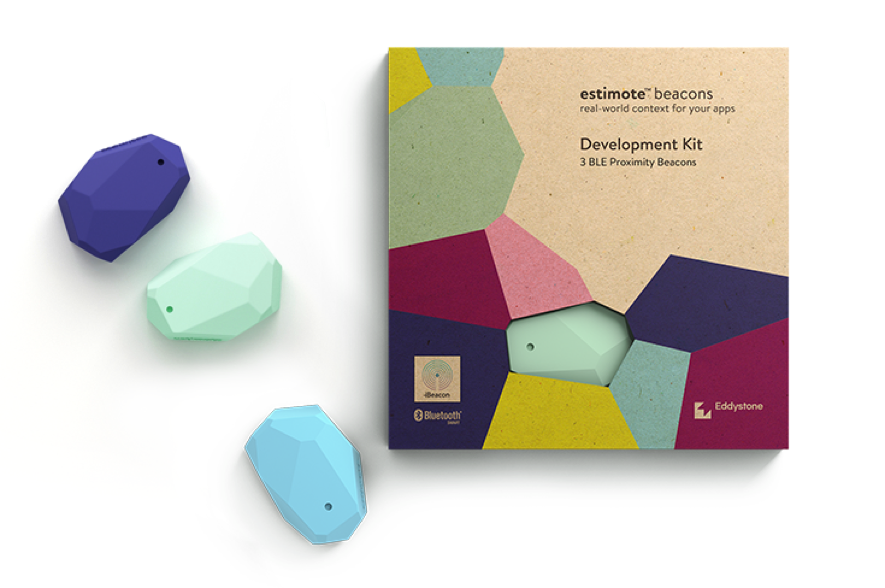
\includegraphics[width=0.6\textwidth]{Figures/estimote_data.png}
  \caption[Estimote Proximity Beacons]{Estimote Proximity Beacons.}
  \label{fig:estimotebeacon}
\end{figure}

They have received a lot of criticism related to their beacon’s battery, because once it is exhausted, the device becomes useless.
The Metropolitan Museum of Art, the Cleveland Museum of Art and the Solomon R. Guggenheim Museum in New York are some examples of users of the Estimote’s beacons.

\subsection{Gimbal} 
\label{subsection:gimbal}
Gimbal\footnote{http://www.gimbal.com} was incubated within Qualcomm, the largest producer of mobile semi-conductors in the world. 
The price of Gimbal hardware is very competitive because they charge a monthly active user fee due to the use of the available cloud service functionality that has to be used with their beacons' security protocol. Gimbal proximity beacon series 21 is introduced in Figure~\ref{fig:gimbalbeacon}.

\begin{figure}[!htb]
  \centering
  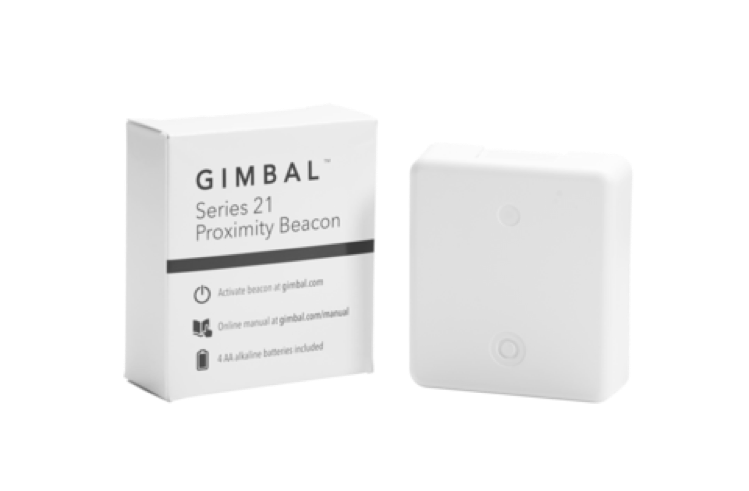
\includegraphics[width=0.6\textwidth]{Figures/gimbal_data.png}
  \caption[Gimbal Proximity Beacon Series 21]{Gimbal Proximity Beacon Series 21.}
  \label{fig:gimbalbeacon}
\end{figure}

This model may not be acceptable to solution builders who simply want high quality hardware and to create their own cloud platform to support a network strategy or a middleware offering. In this case, there may be some challenges in reconciling strategies.
Brands including GameStop and Major League Baseball are among Gimbal’s current customers.

\subsection{Kontakt.io} 
\label{subsection:kontakt}
Kontakt.io\footnote{https://kontakt.io} is an \gls{iot} company and they have focused on monetizing beacon hardware rather than charging for active users. Their image is rooted on cause-based solutions, with a founding story that relates to providing assistance for blind people with beacon-enabled mobile applications. 

The Kontakt.io hardware, shown in Figure~\ref{fig:kontaktbeacon}, is distinguished by a \gls{wi-fi} to Bluetooth gateway or cloud beacon and a robust weather-resistant tough beacon. There are limitations to their beacons’ power options. Their beacons rely on thick coin cell batteries, which limits the battery life to six months when broadcasting at Apple’s prescribed 100ms interval. 

\begin{figure}[!htb]
  \centering
  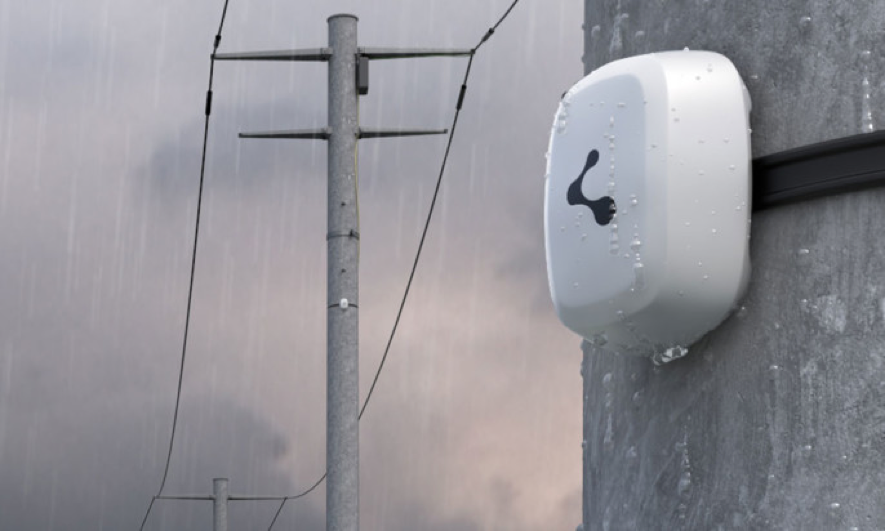
\includegraphics[width=0.6\textwidth]{Figures/kontakt_data.png}
  \caption[Kontakt Beacon]{Kontakt Beacon.}
  \label{fig:kontaktbeacon}
\end{figure}

McDonald’s have recently leveraged a new proximity marketing strategy at 15 McDonald's Cafés in Istanbul, Turkey, sending beacon-enabled promotions to customers within its venues via a mobile application, resulting in a conversion rate of 20 percent.

\subsection{Iotton} 
\label{subsection:iotton}
Iotton~\footnote{http://iotton.com} call themselves a Smart \gls{iot} Solution Provider. They have their headquarters in China and sell \gls{iot} solutions for the rest of the World from online sales sites.
Due to the location where the beacons are produced and their beacons' simple model, presented in Figure~\ref{fig:iottonbeacon}, Iotton can sell very low cost beacons, even if they often have to send the beacons far away, making the users pay for the shipment

\begin{figure}[!htb]
  \centering
  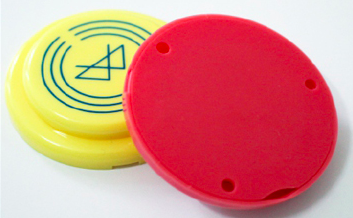
\includegraphics[width=0.4\textwidth]{Figures/iotton_data.png}
  \caption[Iotton's beacon tag]{Iotton's beacon tag.}
  \label{fig:iottonbeacon}
\end{figure}

\subsection{Shenzhen Sky Electronics Manufactory} 
\label{subsection:shenzhen}
Shenzhen Sky Electronics Manufactory is a manufacturer company with their headquarters in Guangdong, China. 
Their beacons have a visual very close to the Estimote beacons but they provide the user the possibility of removing the battery and replace it with a new one, which is an advantage. In Figure~\ref{fig:shenbeacon} it is possible to see how the battery can be removed.

\begin{figure}[!htb]
  \centering
  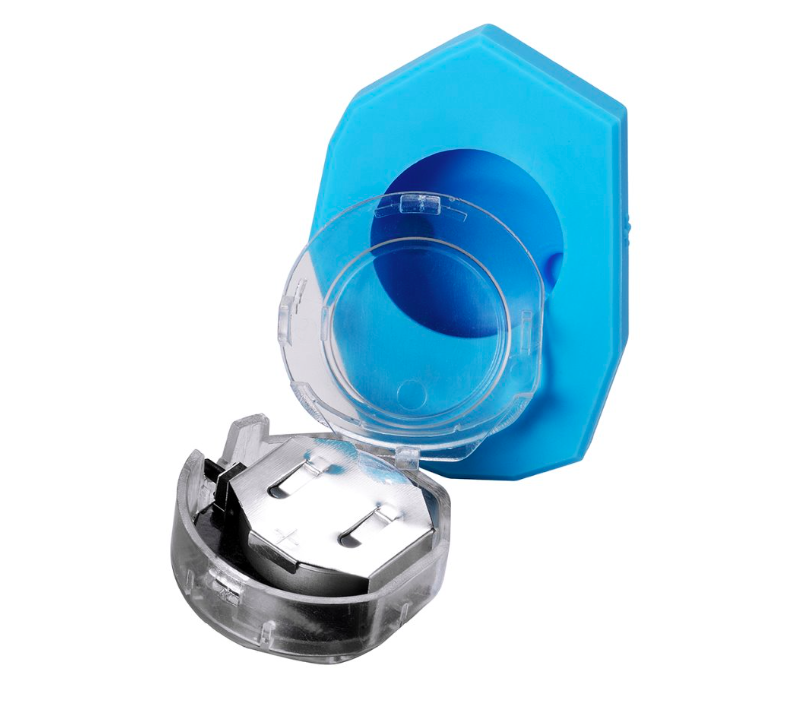
\includegraphics[width=0.5\textwidth]{Figures/shen_data.png}
  \caption[Shenzhen Sky Electronics Manufactory's beacon]{Shenzhen Sky Electronics Manufactory's beacon.}
  \label{fig:shenbeacon}
\end{figure}


\subsection{Comparison} 
\label{subsection:comparison1}

In short, it is possible to combine the characteristics of the beacons from the most known beacon manufacturers, such as: cost, range, battery life and if the battery is rechargeable or not. These features are compared in the Table~\ref{tab:manufdif}. 

\begin{table}[!htb]
  \renewcommand{\arraystretch}{1.5} % more space between rows
  \centering
  \resizebox*{\textwidth}{!}{
  \begin{tabular}{lccc p{1.5cm}}
    \toprule
   \textbf{ Beacons      } &Estimote Proximity Beacons&Gimbal Proximity Beacon Series 21&Kontakt.io Beacon\\
    \midrule
    \textbf{Manufacturer}    &Estimote&Gimbal&Kontakt.io \\
    \textbf{Price }			&\$59 - 3 beacons&\$30.00 - 1 beacon&\$60.00 - 3 beacons\\
    \textbf{Range}	&70m&50m&70m\\
    \textbf{Battery life}  &\begin{tabular}[t]{@{}c@{}}24 months, can change depending on\\ the use of their Smart Power Mode \end{tabular}&18 months, transmitting every 100ms&\begin{tabular}[t]{@{}c@{}}24 months transmitting every 350ms or\\ 6 months transmitting every 100ms\end{tabular}\\
    \textbf{Rechargeable	}	&No&Yes, four standard AA alkaline batteries&Yes\\
    \bottomrule
  \end{tabular}
  }
  \caption[Manufacturers' Beacons Differences]{Manufacturers' Beacons Differences.}
  \label{tab:manufdif}
\end{table}

It is possible to see that the Gimbal's beacon is more expensive than the others because when the user buys a Gimbal's beacon it grants access to their databases using Gimbal's Security Protocol, which requires a monthly fee.

Iotton's IonBeacon Ton9108 costs \$4.69 per unit and the shipment of 10 units with DHL express costs \$21.00 making the total cost of \$67.90, much lower than the cost done by the the manufacturers introduced before, even though it only differs in the battery life and the \gls{tx} interval. Iotton beacon only permits \gls{tx} intervals of 200ms, 300ms, 500ms and 900ms.

Shenzen's beacon costs \$8 per unit and the shipment of 10 units costs with DHL express \$18 making the total cost of \$98, much lower than the previous manufacturers with equivalent characteristics and with the possibility to replace the battery.

All of the manufacturers provide their \gls{api} to change the beacons' power intensity, their interval of \gls{tx} and their \gls{sdk} to the developers.

\section{Applications}
\label{section:aplications}

The market already has several applications related to the beacon positioning. However, most of these solutions can only be used to the purpose they were developed for and the application code is not open to the community. Some of these applications are:
\begin{itemize}
\item Launch Here;
\item Ballpark;
\item San Francisco International Airport.
\end{itemize}

\subsection{Launch Here}
\label{subsection:launchhere}
"Launch Here" application allows the user to automate tasks on its \gls{ios} devices.
Multiple beacons can be place in locals where the user opens the same application or a \gls{url} regularly, so that next time that the user approaches that beacon the Launch Here application will trigger an application or an \gls{url} which is associated with that beacon.

For example, if a beacon is placed near a sofa at home and the user comes near it , Launch Here can launch a journal application. The hour of this notification can be set before it is triggered so that no unwanted notifications happen.
To launch this application, the user needs to have an iBeacon.

As soon as the user is nearby a placed beacon and the screen is unlocked, the application of choice will appear as notification, shown in Figure~\ref{fig:lauchhereapp}, and a simple swipe can launch it.

\begin{figure}[!htb]
  \centering
  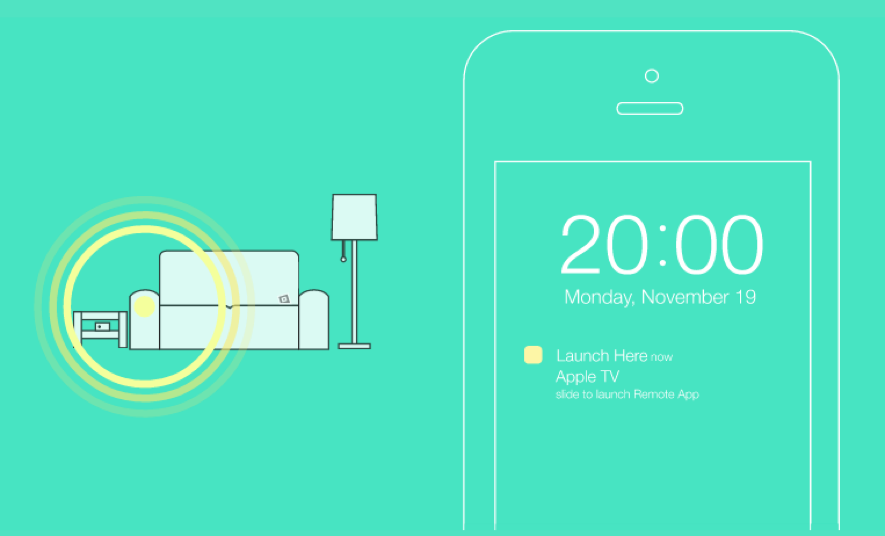
\includegraphics[width=0.6\textwidth]{Figures/launchhere_data.png}
  \caption[Lauch Here Application]{Launch Here Application.}
  \label{fig:lauchhereapp}
\end{figure}

\subsection{Ballpark}
\label{subsection:ballpark}
MLB.com Ballpark application\footnote{http://mlb.mlb.com/mobile/ballpark/}
%, shown in Figure~\ref{fig:ballparkapp}, 
is one of the best applications in the sports domain and has several interesting features, working as follows: when the user loads the application on the way to the stadium, it immediately identifies the stadium and opens information specific to that one. Once near the entrance, it displays the barcode of the user ticket and directs the user to the relevant seat via a map while also highlighting the nearby points of interest.

From the owner of the application point of view, the application can also track the visits made by their fans, enabling them to reward fans with special coupons and discounts for their frequent visits, shown in Figure~\ref{fig:ballparkapp}. 


\begin{figure}[!htb]
  \centering
 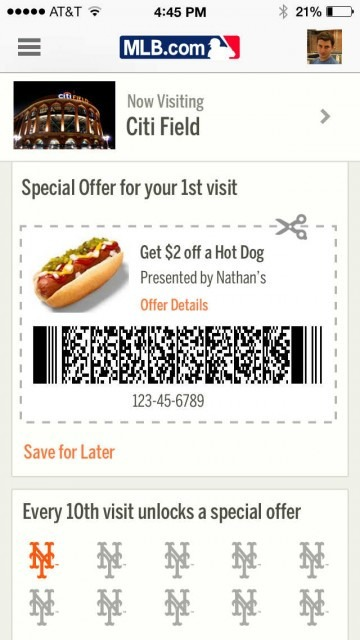
\includegraphics[width=0.35\linewidth]{Figures/ballpark3_data.png}
  \caption[At the Ballpark Application]{At the Ballpark Application.}
 \label{fig:ballparkapp}
\end{figure}


\subsection{San Francisco International Airport}
\label{subsection:sanfrancisco}
San francisco International Airport~\footnote{http://www.flysfo.com/pt} tested a way to help visually-impaired people to navigate around one of their terminals using beacons. These beacons are provided by Indoo.rs an indoor positioning company.
The system uses Apple's Voiceover technology to read out points of interest as they come on screen, meaning that the application could read in the display how to move to the nearest point of interest that appears in the application. In Figure \ref{fig:sanfranapp} a map can be seen in the mobile device.

\begin{figure}[!htb]
  \centering
  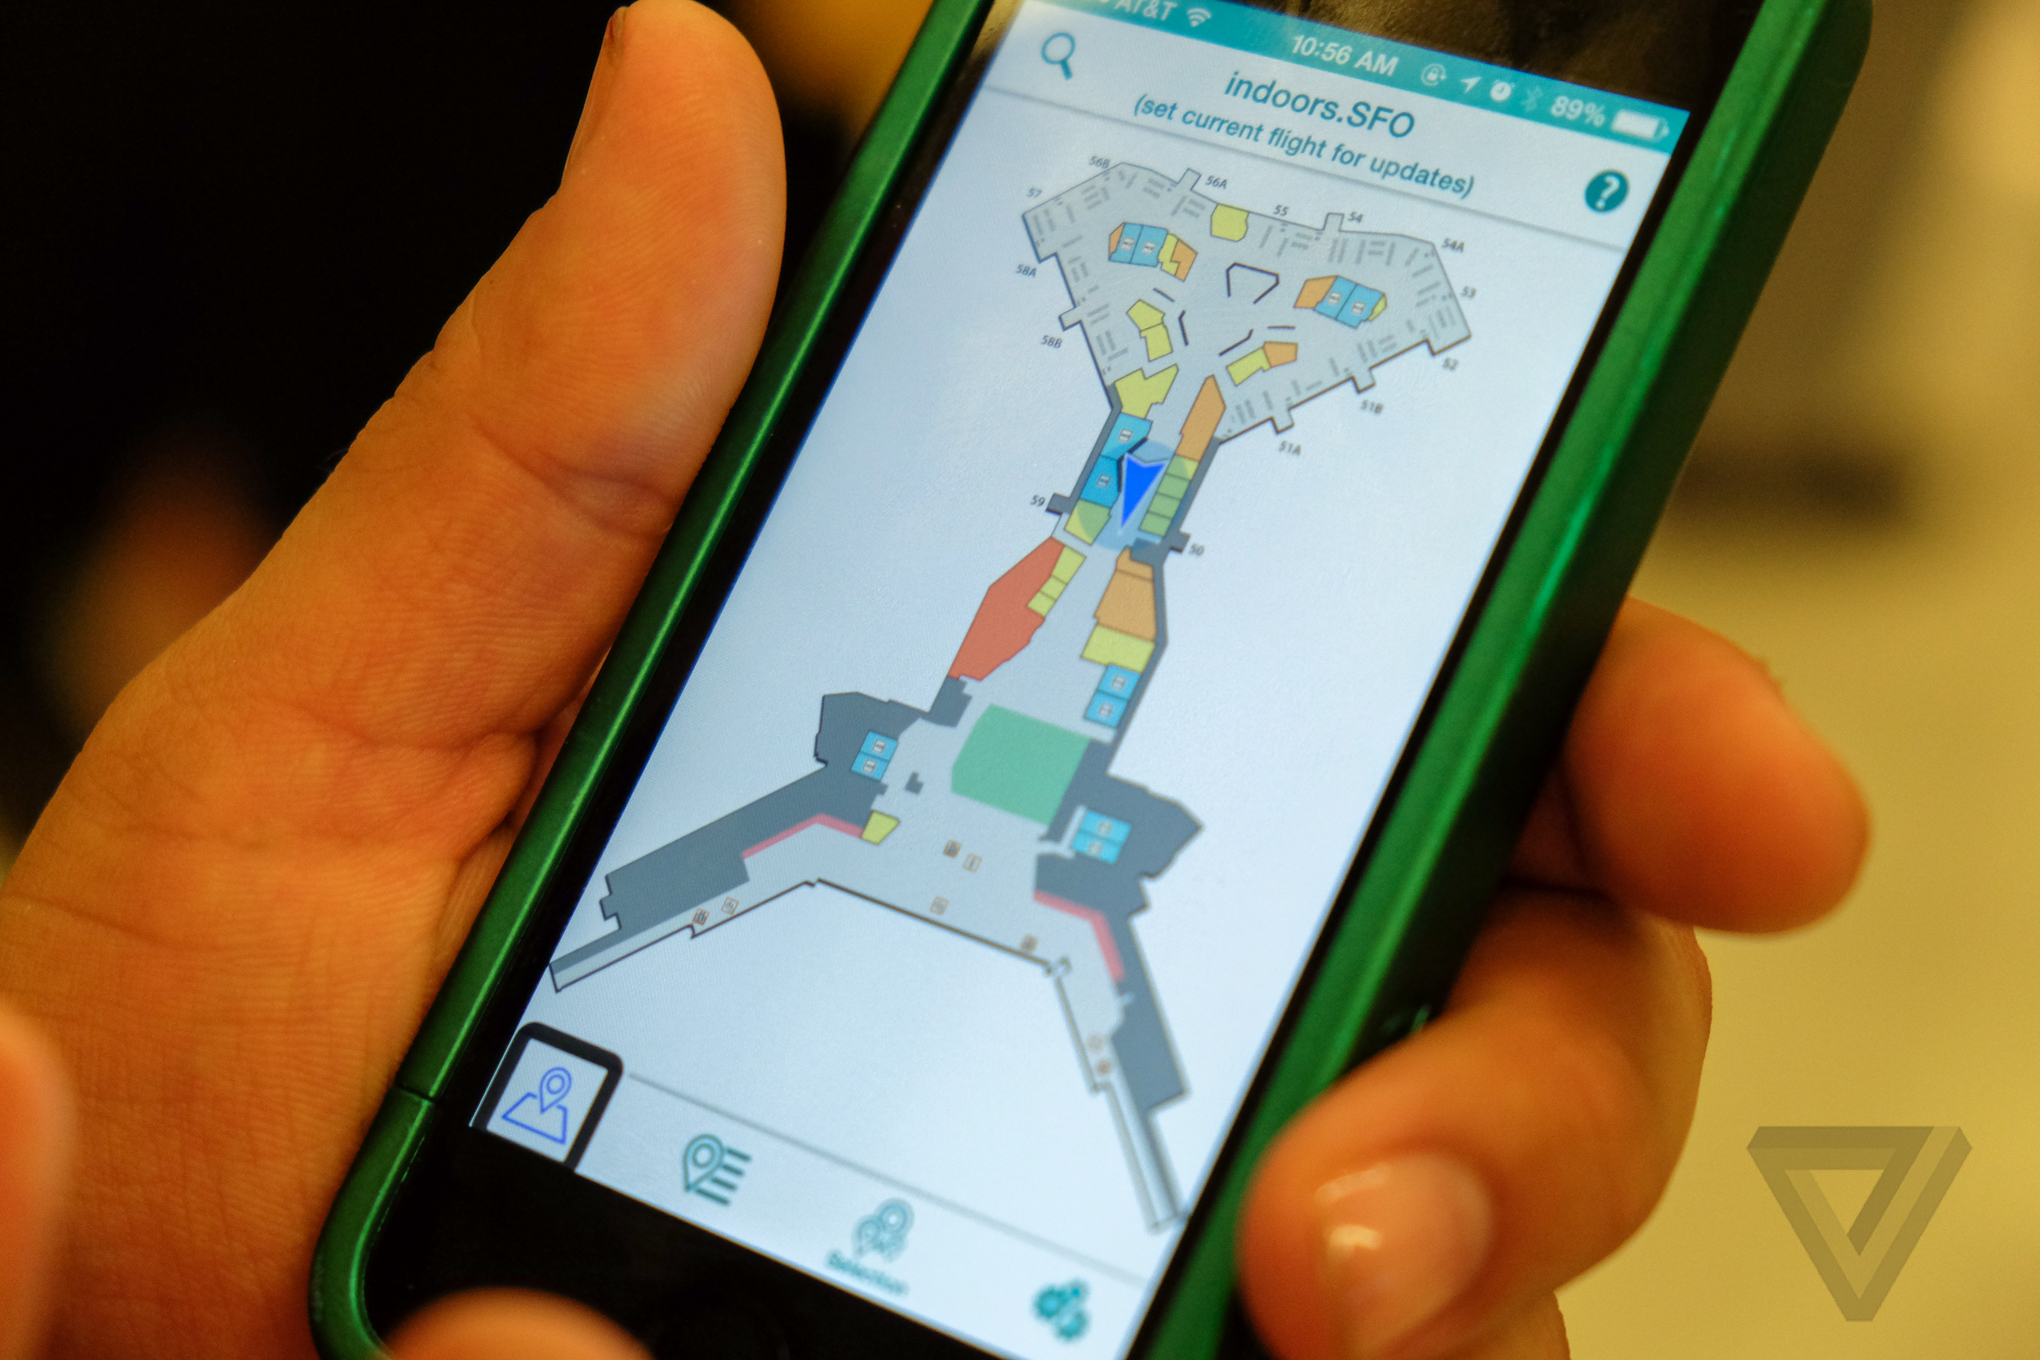
\includegraphics[width=0.6\textwidth]{Figures/sanfrancisco_data.jpg}
  \caption[San Francisco International Airport Map]{San Francisco International Airport Application.}
  \label{fig:sanfranapp}
\end{figure}


In general the applications using beacons are being used to provide the users with the latest promotions or relevant information and welcome them as they enter the owner's store, museum, hospital, restaurant, airport, stadium, etc. 
To the owner of the beacons application, it can inform them where their customers have been, keeping track of them.



\section{Summary}
\label{section:summarybackground}
%%%%%%%%%%%%%%%%%%%
In order to create an indoor system to estimate the position of a mobile device, technologies and methods need to be used or implemented. Cost, accuracy, precision, complexity, scalability and robustness are variables in a technology. \gls{gps}, \gls{wi-fi}, Bluetooth, \gls{qrcodes}, \gls{nfc} and \gls{rfid} are introduced presenting their differences relating the variables mentioned before and their limitations in an indoor environment. \gls{gps} is unsuitable for indoor positioning due to its low accuracy and precision. In some mobile devices is impossible to access the value of \gls{rss} from all access points in the range of the mobile device, making \gls{wi-fi} impossible to use more advanced positioning methods. Bluetooth has a delay due to the transmission intervals of the \gls{ble} devices or beacons. \gls{qrcodes}, \gls{nfc} and \gls{rfid} need the user to be aware of them. 

The measured \gls{rss} can be used to calculate the position of a device using the Friis free space model Equation.
Positioning methods can be active or passive. Active positioning methods determine the position of a device based on the signals received. Proximity sensing, lateration and angulation are all active positioning methods. Passive positioning methods depend in the environment. Fingerprinting is a passive positioning method.

Beacons work following a protocol. iBeacon, AltBeacon, Eddystone and URIBeacon are beacon' protocols. These protocols differ in the advertisement format. iBeacon and AltBeacon broadcast a unique ID number. URIBeacon broadcasts and \gls{url}. Eddystone can broadcast both an ID number or an \gls{url}.

Beacons' manufacturers try to differentiate among others presenting different physical aspects in their hardware, in their software, or in the business aspects that they offer to the user's solutions. Estimote, Gimbal and Kontakt are some of the most well-known manufacturers. They differ in the appearance of their beacons, their battery life and its rechargeability. They offer to their development clients different \gls{sdk}s. Estimote and Kontakt are more common inside developers. Iotton and Shenzhen Sky Eletronics are the cheapest choice when it comes to a beacons solution.

Applications are being developed to welcome the clients by using Bluetooth beacons. To the owner, these beacons can mean the possibility of keeping track of the customers. To the customers, these beacons can represent the possibility of receiving the latest promotions or information relevant to the place where they position.
